In order to perform contact angle measurements on any material, the surface of that material must be pristine and well characterized. There can be no doubt that the probed surface is free of debris, organics, or oxides, for the case of metals, lest the contact angle be influenced by something other than the probed material. Proper sample storage and chemical cleaning (acetone $\Rightarrow$ methanol $ \Rightarrow $ DI rinse $ \Rightarrow $ N$_2$ dry) is satisfactory for removing particulates and organic residue, but exposing a bare metal surface by removing the native oxide layer is challenging. This chapter provides basic oxide removal techniques, but there is a more detailed oxide removal study in Chapter \ref{chapter3}. 
The surface must also be as close to atomically flat as possible. Most literature will approximate their surfaces as flat as long as the roughness is 10$^2$ greater than the contact area radius. 

One of the challenges in developing this new surface energy measurement capability is the need to expose the surface of the metal substrate that is shielded by surface oxides. The following strategies for removing the oxide layer and preventing  natural oxidation, thereby increasing the accuracy of measurement, will be employed independently and in combination:
\begin{outline}
	\1 A flux used in high-temperature metal joining processes plays roles of dissolving of the oxides on the metal surface and preventing of re-oxidation as a chemical agent.
	\1 Colloidal silica polishing with nano-sized particles, such as is used for precise surface observations, like EBSD scans, which require clean surfaces to accurately detect patterns.
	\1 Electro-polishing is effective for passivation of clean surfaces after chemical and mechanical polishing for removal of surface oxides. 
\end{outline}
%Results using the proposed approach were to be validated through comparison of results for oriented single crystals with published theoretical values for pure metal elements of a specific crystallography (e.g. Ni, Cu, Fe)  and comparison with experimental data from amorphous metals (e.g. Vitreloy or liquid steel) with destructive high temperature methods for measuring surface energy. 
It should be noted that all of these techniques will not prevent oxides from forming for an extended period of time. Therefore, the cleaning would have to be followed by isolation in high vacuum, an inert environment, or another liquid environment that prevents oxidation.

\subsection{Sample Preparation}
\subsubsection{Rolling and annealing}
Single crystal ingots were prepared by DOE Ames Laboratory, most likely using the Czochralski Method. Polycrystalline samples are prepared in the Aerosmart lab by Dr. Suok-Min Na using a progressive hot, warm, then cold rolling technique from a polycrystalline Galfenol ingot. The annealing process is described in \hyperlink{abnormal-grain-growth}{Chapter 1}. Single crystal samples are preferred for contact angle experiments because the prepared surface is isotropic, therefore multiple locations on a single sample surface can be probed and compared as equal surfaces. 


\subsubsection{Polishing}


Samples were prepared by manual grinding with incrementally higher grit SiC paper up to 1200 fine grit and then fine polishing using silica gel with 60 nm sized particles to minimize the roughness as well as the stressed surface states created during grinding.\cite{Hoffmann1987} Roughness measurements were performed on ten different 1$\mu$m x 1$\mu$m areas with an atomic force microscope (Veeco Dimension 3100) after fine polishing. Surface roughness values of ~1 nm were measured, thus there is minimal roughness influence on the contact angle measurements. Below are AFM images showing the difference between 1200 fine polishing and subsequent silica gel polishing. 
\begin{figure}
	\centering
	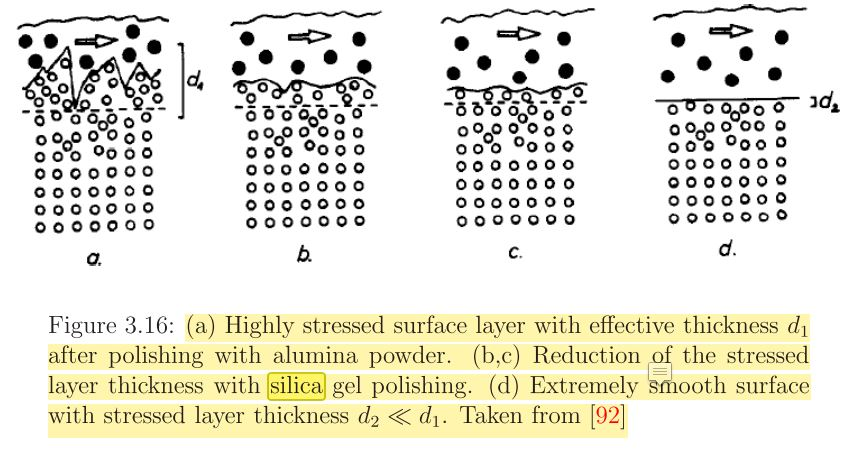
\includegraphics[width=\linewidth,trim={0 0 0 1cm}]{silica-polish}
	\caption{}
	\label{fig:silica-polish}
\end{figure}


%TODO insert an AFM image here to show roughness after a silica polish



\subsubsection{Electron Backscatter Diffraction}
%TODO Insert highly-textured polycrystal sample EBSD image made near beginning of project. 

%TODO single crystal EBSD images for (100), (110), and (111) samples that were vibratory polished
\subsubsection{Atomic Force Microscopy}
%TODO Expand on why AFM is a good enough calculator of roughness at a nanoscale. 

AFM is one of the simplest ways to determine roughness at the sub-nanometer scale, as opposed to profilometry which tends to lack the $<$100 nm resolution.

\subsection{Thermal Chamber Design Progression}
\subsubsection{Contact Angle Goniometer (Verison 1)}
Preliminary designs of my contact angle goniometer implement a radiative temperature control box which encloses an argon gas filled container where the sample resides, as seen in Figure \ref{fig:rad-temp-box}.  The presence of argon is meant to prevent any further oxidation of the Galfenol sample as well as the gallium droplet. The container was initially made of a clear acrylic plastic, but prolonged exposure to temperatures above 80\degree C caused thermal deformation of the plastic making longer experiments impossible to perform without environment contamination.  A clear pyrex container replaced the acrylic box to fix this issue.  Application of the liquid gallium drop to our surfaces was done via a mounted plastic syringe with disposable stainless steel hypodermic needles that were available at the time. Liquid gallium tends to adhere strongly to the stainless steel needle tips which makes wetting to the sample very difficult. The stainless steel tip tends to deform the highly viscous gallium drop resulting in non-uniform hemispheric drop shapes, as shown in Figure \ref{fig:deformed-ga}.
\begin{figure}[h]
	\centering
	\begin{subfigure}[c]{0.45\textwidth}
		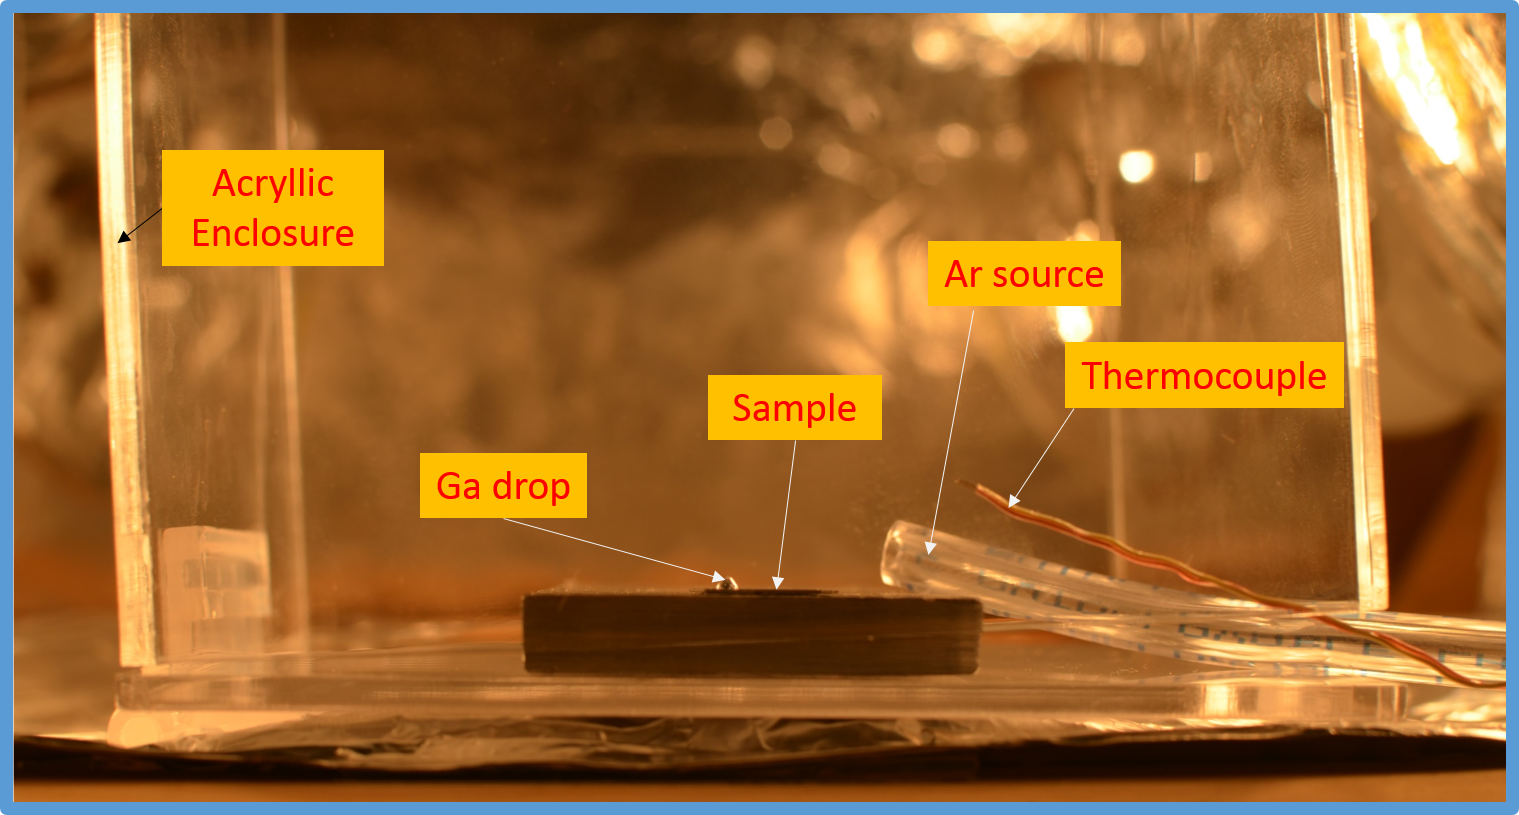
\includegraphics[width=\linewidth]{rad-temp-box}
		\subcaption{~}
		\label{fig:rad-temp-box}		
	\end{subfigure}
	\begin{subfigure}[c]{0.45\textwidth} 
		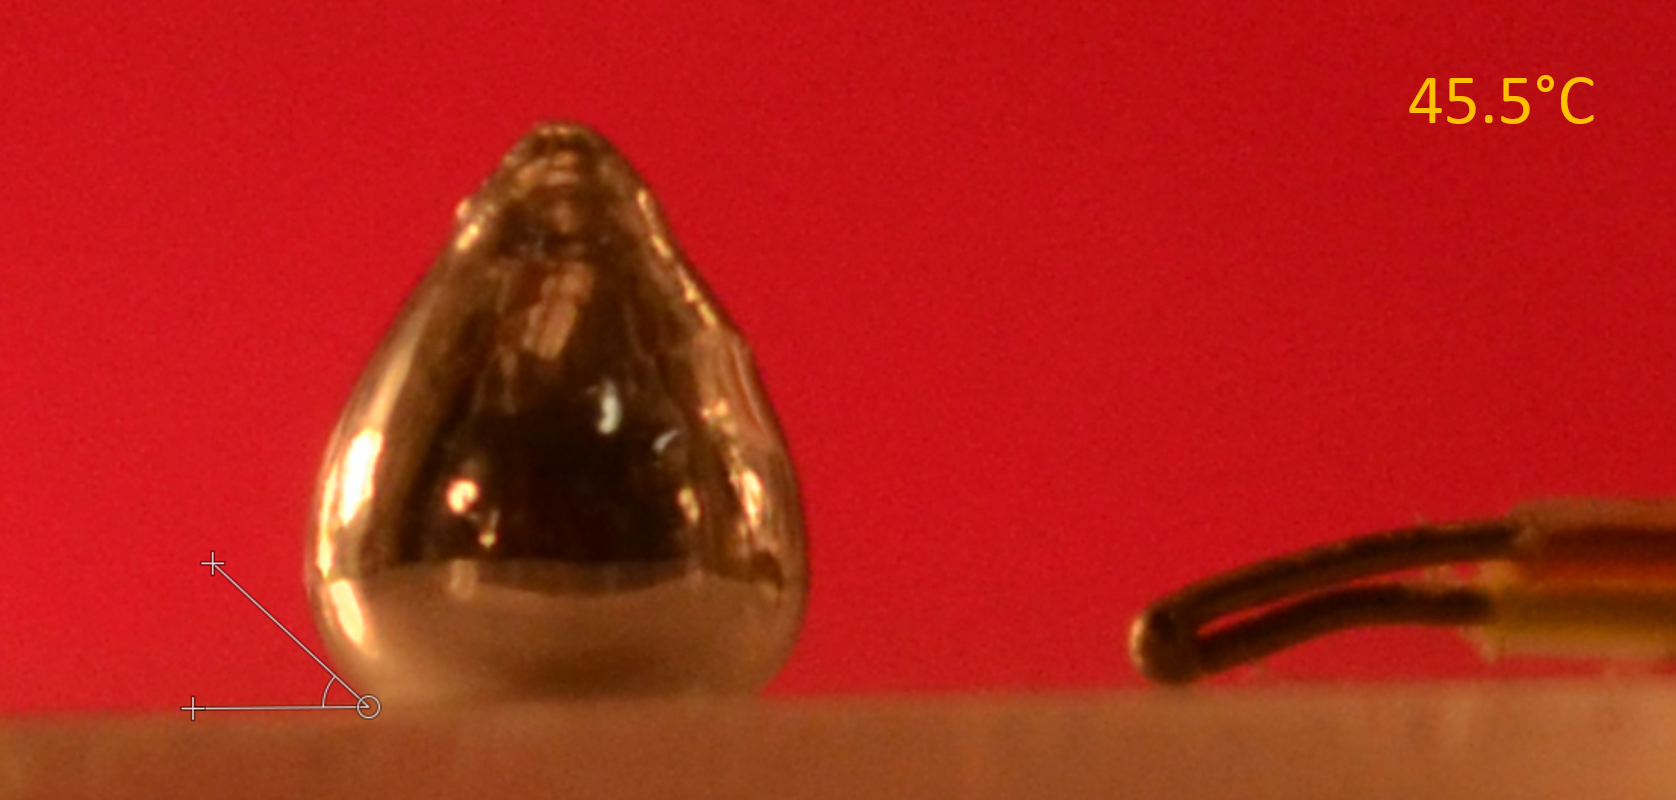
\includegraphics[width=\linewidth]{deformed-ga}
		\subcaption{~}
		\label{fig:deformed-ga}		
	\end{subfigure}
	\caption{(a) The first design of our contact angle goniometer.  The acrylic container houses the argon environment and sample.  This design was modified with a more stable glass enclosure. (b) A highly deformed gallium drop next to the thermocouple on a ceramic YAG test sample at 45.5\degree C. The angle measured on this droplet was subtracted from 180\degree since it was not measured through the liquid.}
	\label{fig:prelim-design}
\end{figure}



%\begin{figure}
%	\centering
%		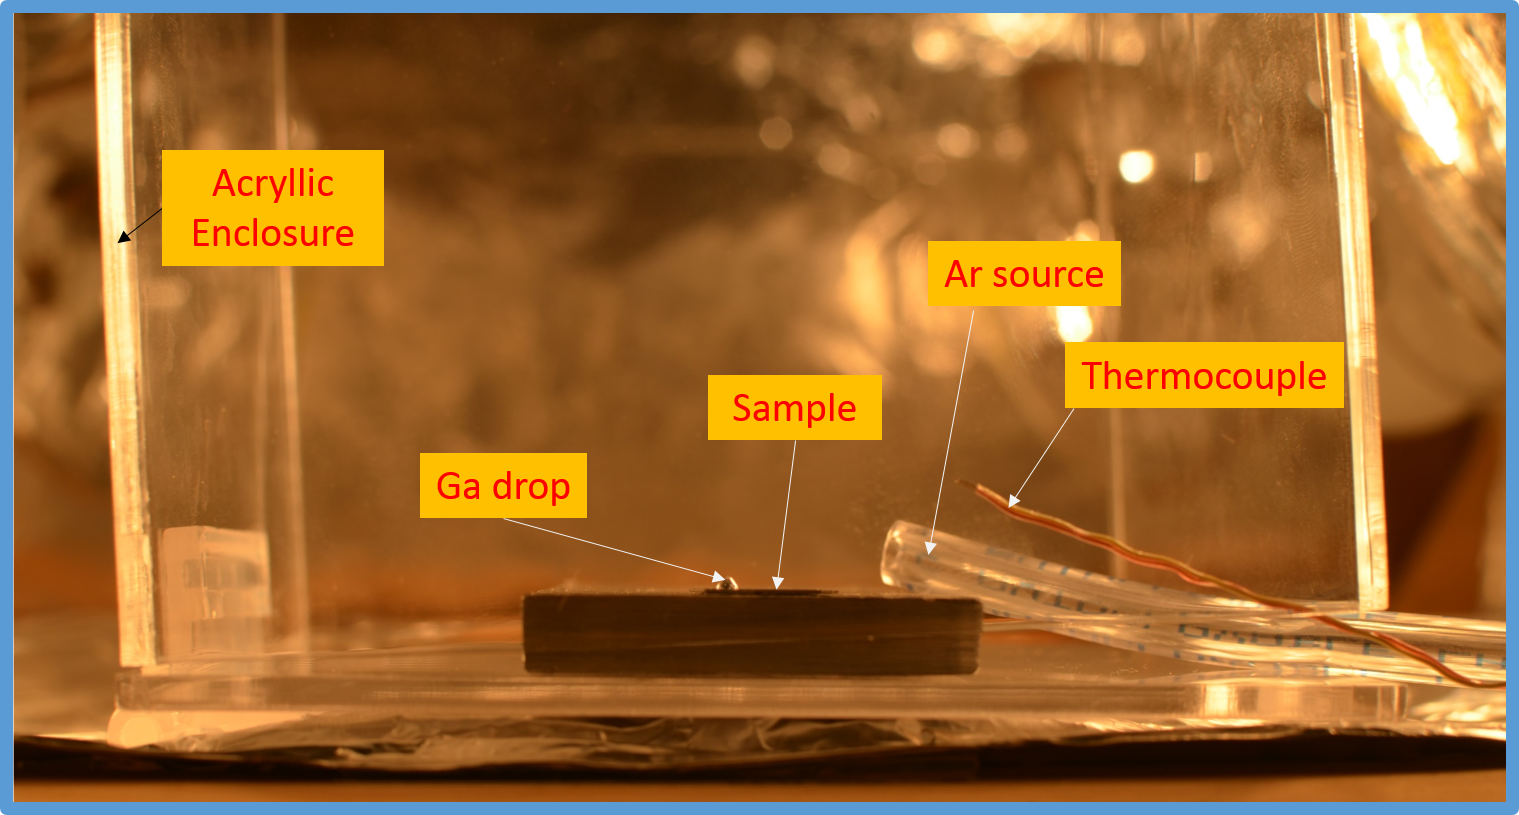
\includegraphics[width=\linewidth]{rad-temp-box}
%	\caption{(a) The first design of our contact angle goniometer.  The acrylic container houses the argon environment and sample.  This design was modified with a more stable glass enclosure. (b) A highly deformed gallium drop next to the thermocouple on a ceramic YAG test sample at 45.5\degree C.}
%	\label{fig:prelim-design}
%\end{figure}
The radiative box that housed this experiment had a high variability in temperature according to thermocouple readings, so a smaller apparatus with a top-side syringe opening is made to properly perform gallium drop tests at specific temperatures and prevent interaction with the experiment environment. There must also be bright white backlighting to obtain a high contrast drop profile. In this radiative box configuration, the high-reflecting liquid metal surface prevents a high contrast drop profile image, as seen in Figure \ref{fig:deformed-ga}. Proper contact angle measurements also require the gallium droplets to carefully wet the surface while forming an axisymmetric and spherical-like shape on the solid surface. A height adjustment system must be used to move the gallium pendant drop close enough to the sample surface for solid adhesive forces to overcome the adhesion to the needle. Lastly, the argon gas environment could be more well contained, instead of just filling up the glass sample enclosure from the bottom and spilling out the top due to higher density argon displacing the surrounding air environment. 

\subsubsection{Version 2}
\begin{figure}
	\centering
	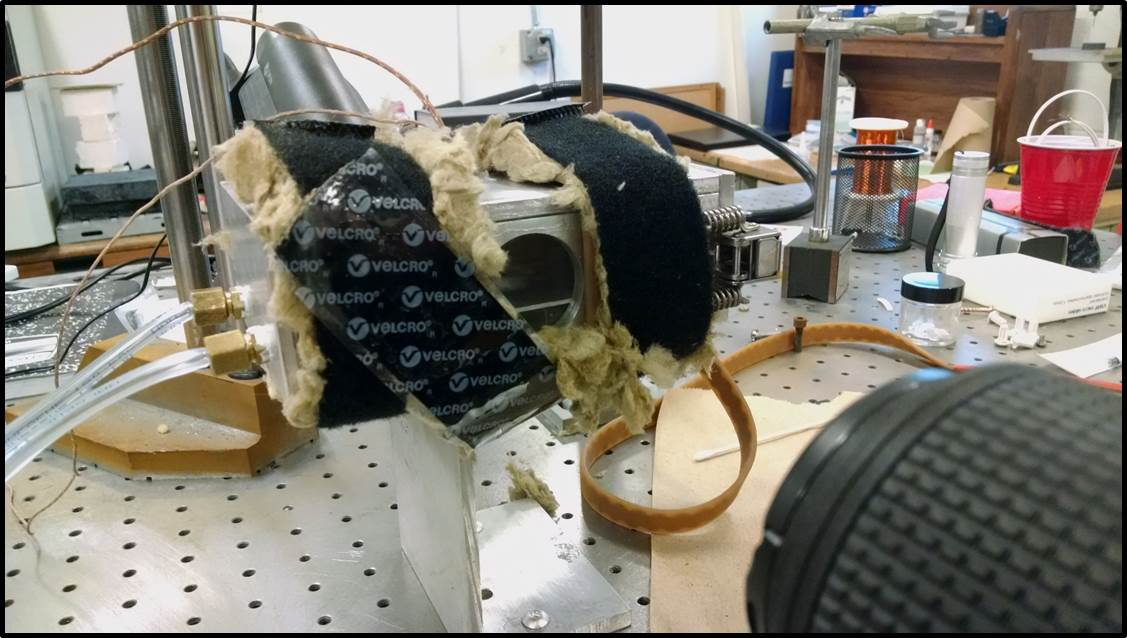
\includegraphics[width=\linewidth,trim={0 0 0 1cm}]{enviro_chamber}
	\caption{The second version of our gallium contact angle goniometer. The aluminum enclosure conductively transfers heat, the gas lines flow Ar gas into the chamber, top-mounted thermocouples monitor the gas and sample temperature, and the glass windows allow for backlighting of the drop profile along with high resolution image capture using a DSLR camera.}
	\label{fig:enviro_chamber}
\end{figure}
The new experimental apparatus can be seen in Figure \ref{fig:enviro_chamber}. The main structure is made of aluminum with two round glass windows on the front and back. The aluminum is meant to conductively transfer heat to the substrate by means of a heating cable wrapped around the outside of the structure. The high thermal conductivity of aluminum allows for a quick transfer of heat, thus an increased control of sample temperature. The time percentage dial controller attached to the heating tape is calibrated with the sample temperature using a thermocouple placed on the sample surface. Sample temperature can be consistently controlled with $\pm$0.5\degree C accuracy. Backlighting greatly improved the drop profile contrast by having only one white light source coming from one side of the droplet, as seen in Figure \ref{fig:deformed_ga}. The Ar environment is also far more contained and controlled. The silicone sealant creates a nearly air-tight system where the Ar gas will displace all gas contaminants that could further oxidize the sample or gallium droplet. 
%These precautions are suitable for any metals samples tested because each sample is polished according to the procedure described above and then cleaned with acetone to remove any oxides. 
Once the sample is inserted and sealed in the environmental chamber, Ar gas prevents further oxidation throughout the experiment. A positive partial pressure is achieved in the chamber with an in- and out-valve to constant flow air out of the chamber.  
A high quality macro lens (Nikon AF Micro Nikkor 200-mm 1:4 D) is used to precisely quantify dimension changes in substrate and liquid metal drop during thermal expansion. 
\begin{figure}
	\centering
	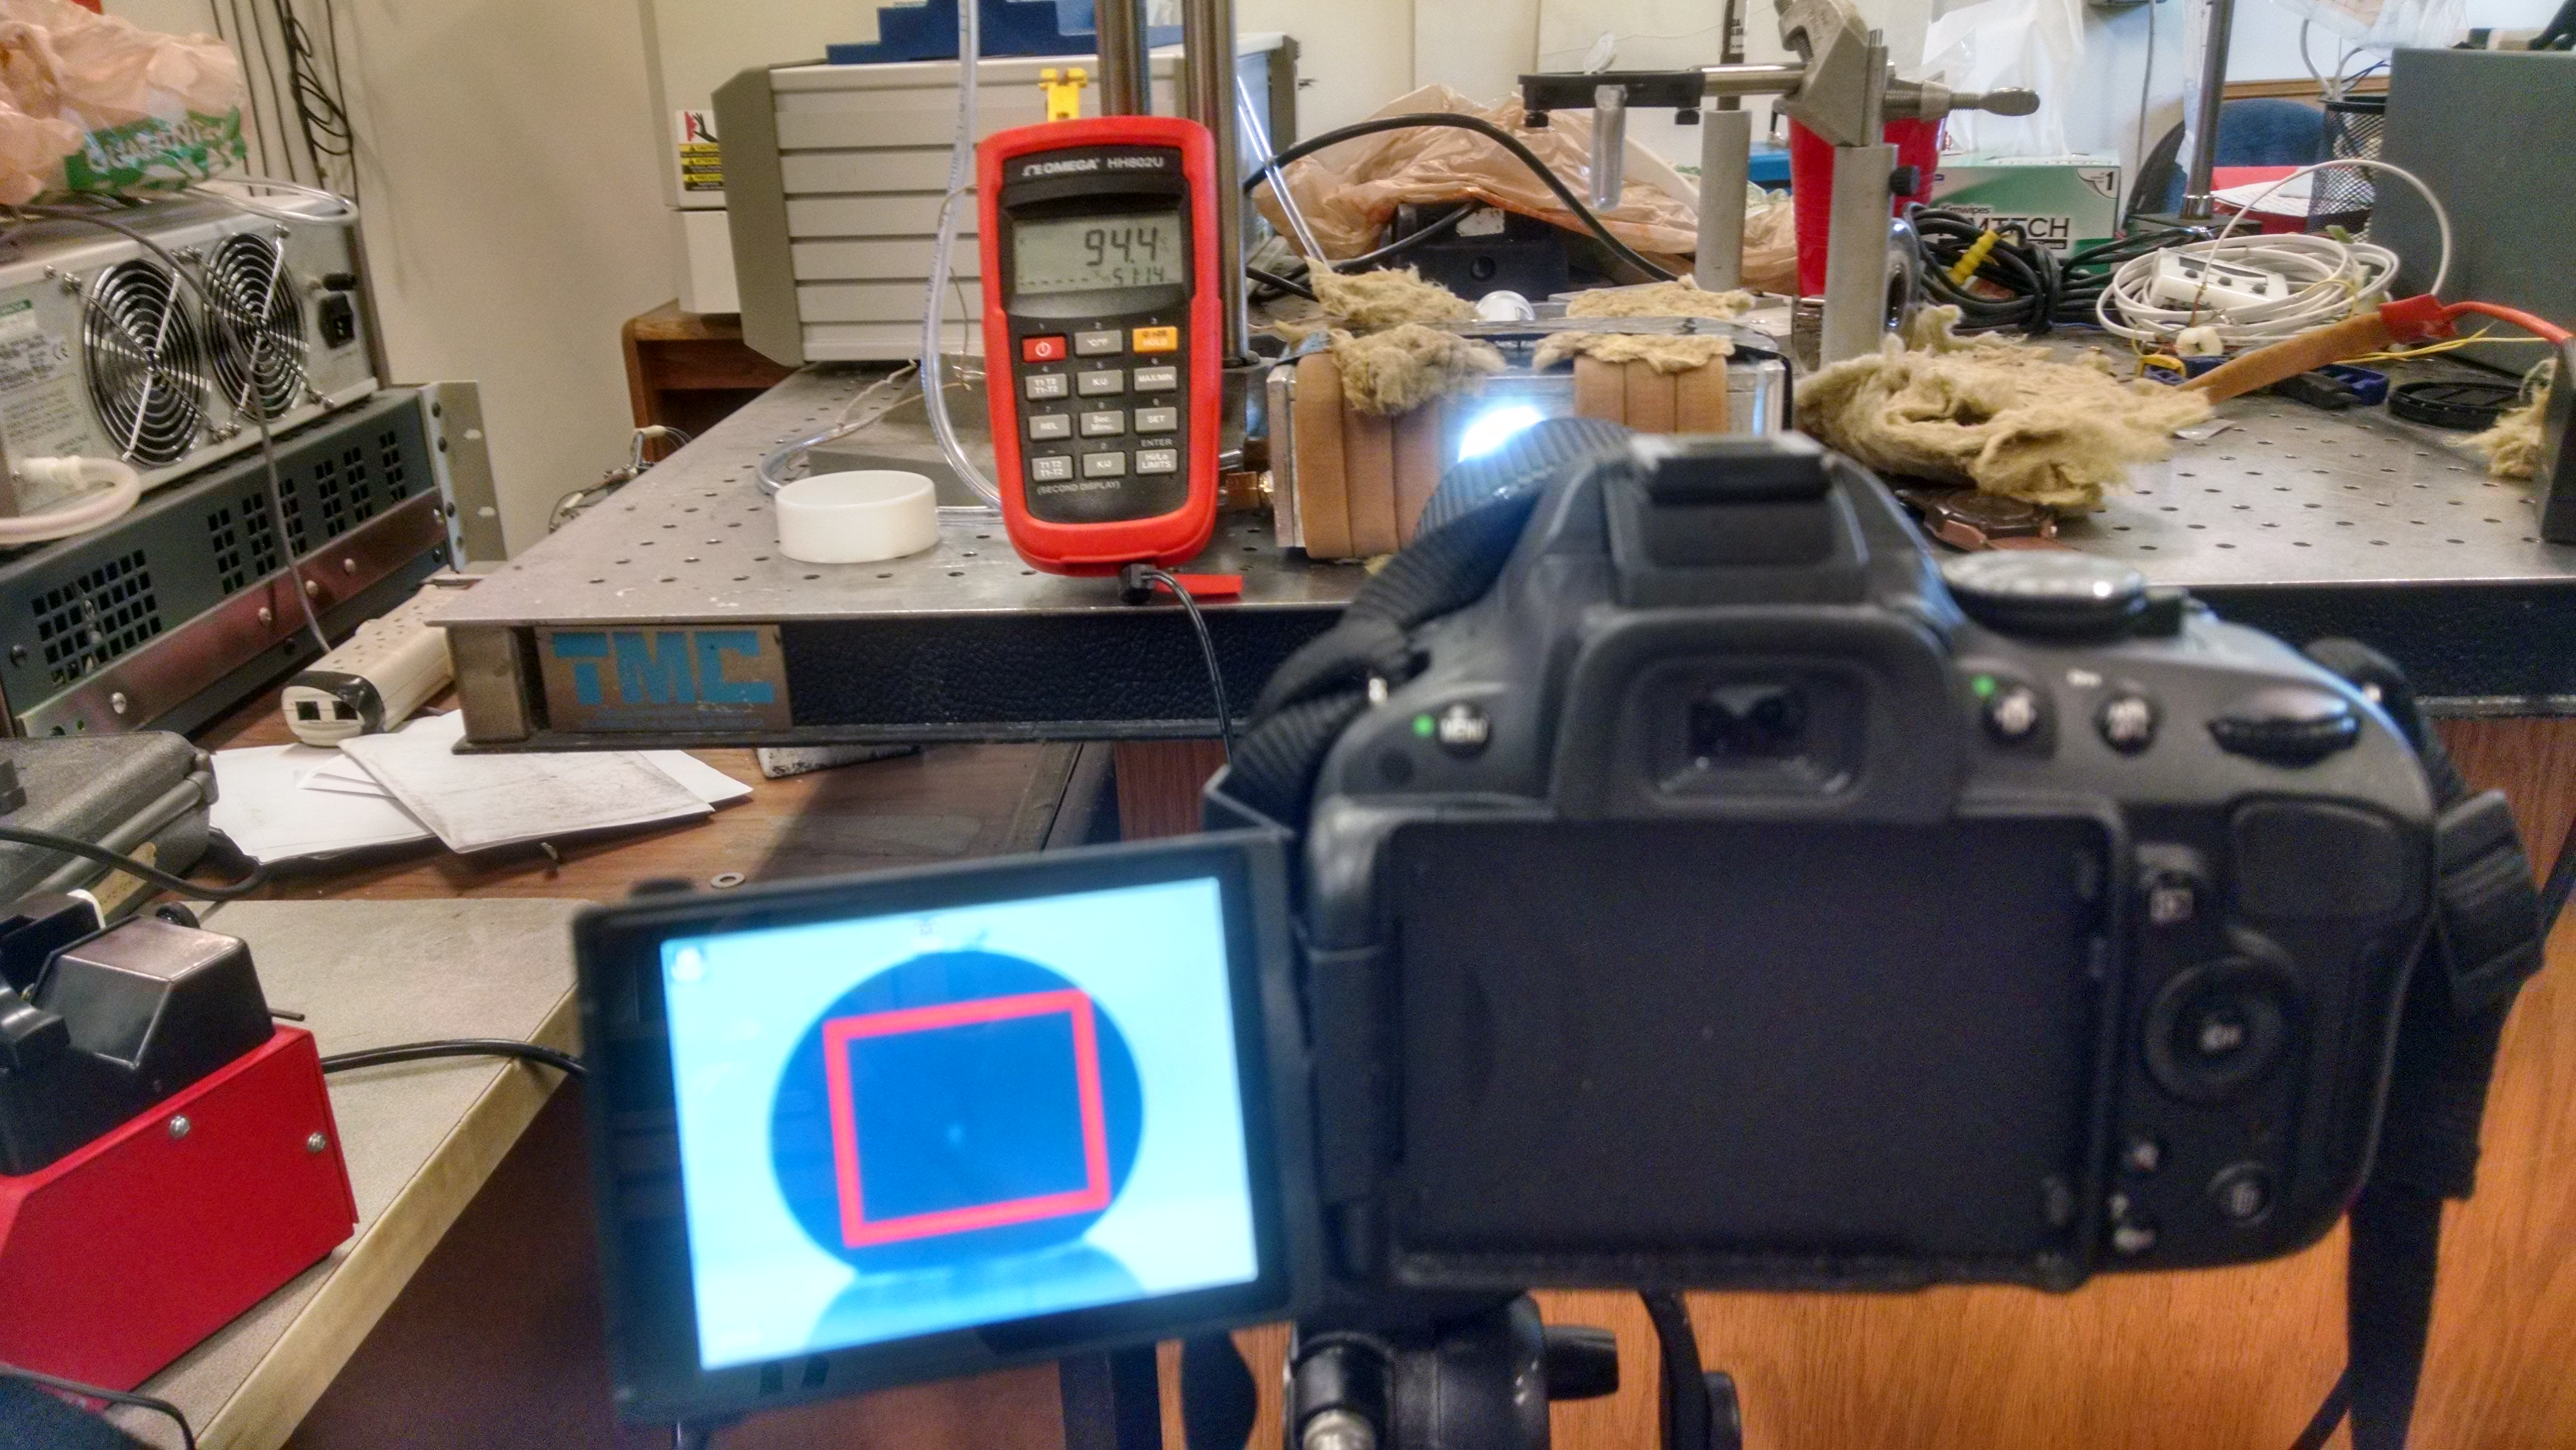
\includegraphics[width=\linewidth,trim={0 0 0 1cm}]{DSLRcamera}
	\caption{This is a photograph of a picture being taken of a gallium droplet on highly-textured polycrystalline at 94.4\degree C (seen from thermocouple meter) using a Nikon DSLR camera with a long macro-lens. }
	\label{fig:DSLRcamera}
\end{figure}

\subsection{Gallium Oxide removal}


While extensive steps have been taken to inhibit oxidation on the metal surfaces, preventing oxidation on the surface of liquid gallium was a greater challenge. Pure gallium and Gallium-based alloy surfaces very quickly oxidize in ambient air environments, and form turning a thin layer of gallium oxide (Ga$_{2}$O$_{3}$ and Ga$_{2}$O).\cite{Regan1995,Regan1997,Scharmann2004} Like any other metal, Ga has a high potential for spontaneous oxidation, or passivation. This oxide layer is solid and remains elastic until it experiences a yield stress. Therefore, that an oxidized gallium droplet does not behave as a simple liquid, but as a viscoelastic material. In addition, the oxide layer of gallium is known to adhere to almost any solid surface, causing a severe stiction problem that interferes with interfacial energy measurements.\cite{Scharmann2004}. This shows how dramatically the gallium surface tension decreases when the oxide forms. Khan \etal showed that gallium oxide forms hydroxyl groups on their exterior surface, making the drops lyophilic as opposed to the expected lyophobic behavior of pure gallium, a high surface tension liquid.\cite{Hardy1985,Alchagirov2005} 

\begin{figure}
	\centering
	\begin{subfigure}[c]{0.45\textwidth}
		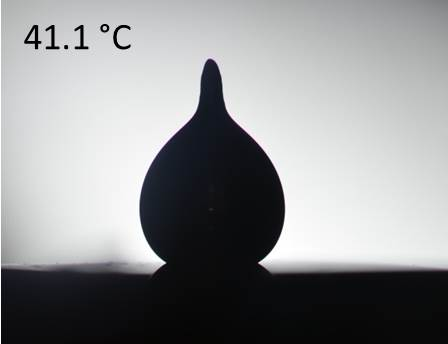
\includegraphics[width=\linewidth,trim={0 0 0 0}]{ga_41c}
		\subcaption{~}
		\label{fig:ga_41c}		
	\end{subfigure}
	\begin{subfigure}[c]{0.45\textwidth} 
		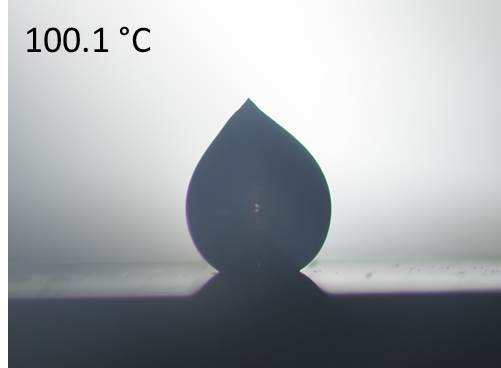
\includegraphics[width=\linewidth,trim={0 0 0 0}]{ga_100c}
		\subcaption{~}
		\label{fig:ga_100c}		
	\end{subfigure}
	\caption{Pure liquid gallium obtains viscoelastic properties when trace amounts of oxygen are present via formation of oxide shell. Non-axisymmetric Ga drops form on this iron substrate.}
	\label{fig:deformed_ga}
\end{figure}
Figure \ref{fig:deformed_ga} shows our direct observation of this phenomenon with teardrop shaped droplets formed by adhering to the iron surface while simultaneously being pulled upwards by the deposition needle. The general shape of these drops were unchanged for many hours even at temperatures approaching $\sim$100\degree C, thus exhibiting the stability of viscoelastic properties caused by the solid oxide layer. Removing the oxide layer from liquid gallium will return normal liquid properties to gallium and allow the use of axisymmetric drop analysis calculations: Young-Laplace equation, tangent method, and circle approximation method. 

Oxide removal permits liquid gallium to directly interact with metal surfaces instead of gallium oxide; the derived terms for \gamSL and \gamLV in Equation \ref{youngs-eqn-ga} become more robust. A number of techniques have been developed to remove and recover gallium oxide on liquid gallium: ultra-high vacuum (UHV) techniques,\cite{Regan1995,Regan1997} chemical vapor etching,\cite{Kim2013,Doudrick2014} and electrohydrodynamic phenomena.\cite{Khan2014} A chemical vapor etch is the best option for this experiment because it has a minimal effect on the surface of metals and the experimental apparatus does not need to be changed.  
To execute the vapor etch, a pendant drop of gallium was formed and a pipette of 37wt\% HCl was brought in close proximity to etch away the oxide layer. The same procedure was performed on the sessile drop of gallium on the desired surface to etch away any oxide left on top of the droplet, as seen in Figure \ref{fig:hcl_vapor_treat}. The contact angles of gallium on bare glass before and after HCl vapor treatment are similar to respective contact angle values in Kim \etal\cite{Kim2013}

The HCl vapor etch may even have the benefit of removing any native iron oxides (Fe$_2$O$_3$) from the FeGa surface itself since HCl is a known etchant of Fe$_2$O$_3$.\cite{Walker1991}



\begin{figure}
	\centering
	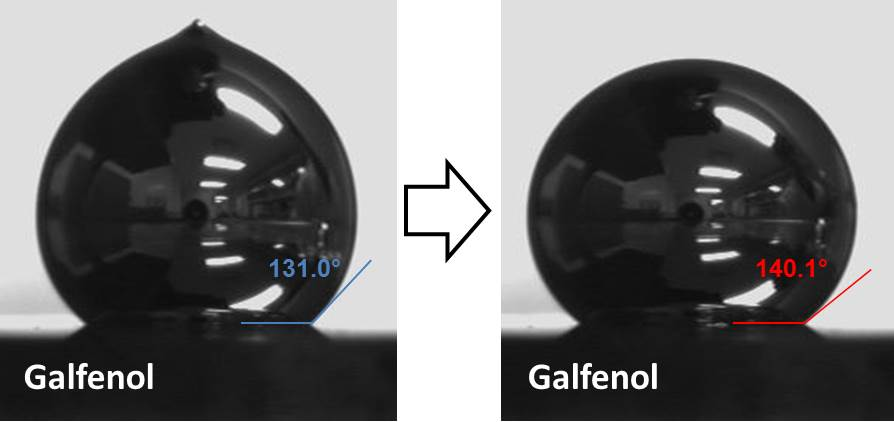
\includegraphics[width=\linewidth,trim={0 0 0 1cm}]{hcl_vapor_treat}
	\caption{This image shows the contact angle of gallium on a Galfenol sample in an argon environment before and after HCl vapor treatment.}
	\label{fig:hcl_vapor_treat}
\end{figure}





